\ifsolo
    ~

    \vspace{1cm}

    \begin{center}
        \textbf{\LARGE Intégration sur un intervalle quelconque} \\[1em]
    \end{center}
    \tableofcontents
\else
    \minitoc
\fi
\thispagestyle{empty}

\ifsolo \newpage \setcounter{page}{1} \fi

\section{Rappels}

L'opération d'intégration sur $\CPM([a, b], \mathbb R)$ est linéaire positive croissante. On a \[
    \left| \int_a^bf \right|\leq \int_a^b|f|\leq (b-a)\sup_{[a,b]} |f|
\]
et similairement \[
    \left| \int_a^bfg \right|\leq \sup_{[a,b]}|f|\int_a^b|g|
\]
Si $f$ est continue alors \[
    \left| \int_a^bf \right|=\int_a^b|f|\iff f\text{ de signe constant }
\]
et si $g$ est continue positive, \[
    \inf_{[a,b]}f\int_a^bg\leq \int_a^bfg\leq \sup_{[a,b]}f\int_a^bg
\]
et si $g$ n'est pas identiquement nulle, \[
    \int_a^bg>0\implies \dfrac{\int_a^bfg}{\int_a^bg}\in[\inf f,\sup f]=f([a,b])\implies \exists c, \quad \int_a^bfg=f(c)\int_a^bg.
\]
Le résultat reste vrai si $g$ est identiquement nulle. Si $f$ est continue positive sur $[a, b]$ et $\int_a^bf=0$ alors $f=0$.
Si $f$ et $g$ sont de classe $\mathcal C^1$ alors \[
    \int_a^bfg'=[fg]_a^b-\int_a^bf'g
\]
et si $\varphi:[\alpha,\beta]\to[a,b]$ est $\mathcal C^1$, $f$ continue sur $\varphi([\alpha,\beta])$ alors \[
    \int_{\varphi(\alpha)}^{\varphi(\beta)}f(u)\diff u=\int_\alpha^\beta f(\varphi(t))\varphi'(t)\diff t
\]
Si $f$ est continue par morceaux sur $[a, b]$ alors \[
    \frac1{b-a}\sum_{k=0}^{n-1}f \left( a+k\frac{b-a}n \right)\xrightarrow[n\to+\infty]{}\int_a^bf
\]

\begin{thm}[Taylor avec reste intégral\index{Taylor!formule avec reste intégral}]
    \Hyp $f$ de classe $\mathcal C^n$ sur $[a, b]$
    \Conc \[
        f(b)=\sum_{k=0}^n\frac{f^{(k)}(a)}{k!}(b-a)^k+\int_a^b\frac{(b-t)^n}{n!}f^{(n+1)}(t)\diff t
    \]
\end{thm}

\begin{proof}
    Vu en sup.
\end{proof}

\begin{rem}
    On peut échanger $a$ et $b$ dans la formule.
\end{rem}

\begin{ex}[Irrationnalité de $\cos 1$]
    Supposons $\cos 1=\frac pq\in\mathbb Q$ de sorte que \[
        \cos 1=\sum_{k=0}^q\frac{\cos^{(k)}(0)}{k!}+\int_0^1\frac{(1-t)^q}{q!}\cos^{(q+1)}(t)\diff t\implies0\leq \underbrace{q! \left| \cos 1-\sum_{k=0}^q\frac{\cos^{(k)}(0)}{k!} \right|}_{\in\mathbb N}= \left| \int_0^1(1-t)^q\cos^{(q+1)}(t)\diff t \right|<1
    \]
    donc \[
        \cos 1=\sum_{k=0}^q\frac{\cos^{(k)}(0)}{k!}
    \]
    d'où \[
        \int_a^b\underbrace{(1-t)^q\cos^{(q+1)}(t)}_{\mathcal C^0\text{ de signe constant }}\diff t=0\implies (1-t)^q\cos^{(q+1)}(t)\equiv 0
    \]
    ce qui est aburde.
\end{ex}

\section{Intégrales de Wallis}

On appelle intégrales de Wallis les intégrales \[
    W_n\defeq\int_0^{\frac\pi2}\cos^n\underset{\;u=\frac\pi2-t\;}=\int_0^{\frac\pi2}\sin^n
\]
On a \[
    W_0=\frac\pi2\qquad \qquad \qquad W_1=[\sin t]_0^{\frac\pi2}=1
\]
Pour $n\geq 2$, \[
    W_n=\int_0^{\frac\pi2}\cos \cdot \cos^{n-1}=[\sin\cos^{n-1}]_0^{\frac\pi2}+\int_0^{\frac\pi2}\underbrace{\sin^2}_{1-\cos^2}\cdot~(n-1)\cos^{n-2}=(n-1)W_{n-2}-(n-1)W_n
\]
donc \[
W_n=\frac{n-1}nW_{n-2}
\]
de sorte que \[
    W_{2p}=\frac{(2p)!}{2^{2p}(p!)^2}\frac\pi2\qquad\qquad\qquad W_{2p+1}=\frac{2^{2p}p!^2}{(2p+1)!}.
\]
Pour $t\in [0, \frac\pi2]$, on a $\cos^{n+1}t\leq \cos^nt$ donc $W_{n+1}\leq W_n$. Puis \[
    W_{n+2}=\frac{n+1}{n+1}W_n\leq W_{n+1}\leq W_n \implies \frac{W_{n+1}}{W_n}\xrightarrow[n\to+\infty]{}W_{n+1}\sim W_n.
\]
La suite $((n+1)W_nW_{n+1})_n$ est constante égale à $W_0W_1=W_0$ donc \[
    \frac\pi2(n+1)W_{n+1}W_n\sim nW_n^2\implies W_n\sim\sqrt{\frac{\pi}{2n}}
\]
or \[
    W_{2p}\sim\frac{C\sqrt{2p}(2p)^{2p}e^{-2p}}{2^{2p}C^2(\sqrt pp^pe^{-p})^2}\frac\pi2\sim \frac{\sqrt2}{C\sqrt p}\sqrt{\frac\pi2}\underset{\text{ aussi }}\sim\sqrt{\frac{\pi}{4p}}
\]
donc \[
    C=\sqrt {2\pi}
\]

\section{Fonctions continues par morceaux}

\begin{dfn}[Rappel]\index{continuité par morceaux}
    $f:[a, b]\longrightarrow\mathbb R$ (ou $\mathbb C$) est dite continue par morceaux s'il existe une subdivision finie $\sigma=(a_1, \cdots, a_n)$ ($a_1=a$, $a_n=b$) de $[a, b]$ telle que $f$ est continue sur $]a_n, a_{n+1}[$, et admet une limite à droite et à gauche (ou d'un seul côté aux bords de l'intervalle) en chacun des points de la subdivision.

    L'ensemble de ces fonction est noté $\CPM([a, b], \mathbb R)$
\end{dfn}

\begin{dfn}
    Si $I$ est un intervalle non trivial de $\mathbb R$, on dira que $f$ est continue par morceaux sur $I$ si $f$ est continue par morceaux sur tous segments inclus dans $I$.
\end{dfn}

\begin{ex}
    La partie entière est $\CPM$ sur $\mathbb R$. L'application \[
        x\longmapsto \floor{\frac1x}
    \]
    est $\CPM$ sur $]0, 1]$
\end{ex}

\begin{prop}
    \Hyp $I$ est un intervalle réel non trivial, $f,g\in \CPM(I, \mathbb R)$
    \begin{concenum}
    \item Pour tout $\lambda\in\mathbb R$ (ou $\mathbb C$), $\lambda f+g\in\CPM(I, \mathbb R)$
    \item $fg$ est $\CPM$
    \item $|f|$ est $\CPM$. En particulier, $\max (f,g)$ et $\min (f,g)$ aussi
    \end{concenum}
\end{prop}

\begin{proof}
    On se ramène à un segment de $I$ et c'est vu en sup. \[
        \max(f,g)=\frac{f+g+|f-g|}2
    \]
\end{proof}

\begin{thm}[Rappel]
    \Hyp $f$ continue sur $[a,b]$
   \begin{concenum}
   \item  On note $E(I, \mathbb R)$ l'ensemble des fonctions en escaliers de $I$ dans $\mathbb R$. \[
           \forall \varepsilon>0, \exists \varphi\in E([a, b], \mathbb R), \quad \sup_{[a, b]}|f-\varphi|\leq \varepsilon
       \]
   \item \[
        \exists (\varphi_n)_n\in E([a,b]\in\mathbb R)^{\mathbb R}, \forall n\in\mathbb N^\star, \quad \sup_{[a,b]}|f-\varphi_n|\leq\frac1n
       \]
   \end{concenum}
\end{thm}

\begin{proof}[Idée de la preuve]
    $f$ est uniformément continue (Heine) donc avec une subdivision régulière assez petite on a bien l'approximation.
\end{proof}

\section{Intégration sur un intervalle quelconque}

On note $I$ un intervalle non trivial de $\mathbb R$ et $f\in\CPM(I, \mathbb R)$.

\begin{dfn}
    \begin{enumerate}
        \item Si $I=[a, b[$ avec $b\in\mathbb R\cup \{+\infty\}$, alors \[
                \int_If=\int_a^bf\defeq\lim_{x\to b}\int_a^xf
            \]
            lorsque cette limite existe (on dira alors que l'intégrale est convergente).
        \item Si $I=]a, b[$ alors de même, lorsque la limite existe on définit \[
                \int_If=\int_a^bf\defeq \lim_{x\to a}\lim_{y\to b}\int_x^yf
            \]
            On peut inverser les deux limites car pour $c\in I$, \[
                \int_x^yf=\int_x^cf+\int_c^yf
            \]
        \item Lorsque \[
                \int_I|f|
            \]
            converge, on dit que $f$ est intégrable sur $I$. Si $f$ n'est pas intégrable, on dira que $\displaystyle\int_If$ est semi-convergente si elle converge.
    \end{enumerate}
\end{dfn}

\begin{ex}
    L'application $t\longmapsto e^{-t}$ est $\CPM$ sur $\mathbb R_+$ et \[
        \int_0^x e^{-t}\diff t=1-e^x\xrightarrow[x\to+\infty]{}1\implies \int_0^{+\infty}e^{-t}\diff t=1
    \]
\end{ex}

\subsection{Lien avec les primitives}

Si $f$ est continue sur $[a, b[$ et $F$ est une primitive de $f$, alors pour $x\in[a, b[$, \[
    \int_a^xf=F(x)-F(a)
\]
donc $\int_a^b f$ CV $\iff F$ a une limite finie en $b$.

\begin{ex}
    \[
        \int_0^1\frac{\diff t}{t^\alpha}\text{ CV }\iff t\longmapsto \begin{cases}
            \dfrac{t^{-\alpha+1}}{1-\alpha} &\text{ si }\alpha\neq 1\\\ln|t|&\text{ sinon }
        \end{cases}
        \qquad \text{ a une limite finie en $0^+$ }
        \iff \alpha<1
    \]
    \[
        \int_1^{+\infty}\frac{\diff t}{t^\alpha}\text{ CV }\iff \alpha>1
    \]
\end{ex}

\section{Propriétés algébriques}

\begin{prop}
    \Hyp $f,g\in\CPM(I, \mathbb C)$ telles que $\displaystyle \int_If$ et $\displaystyle \int_Ig$ convergent
    \begin{concenum}
    \item \[
            \forall \lambda\in\mathbb C, \quad \int_I(\lambda f+g)\text{ CV  et }\int_I(\lambda f+g)=\lambda\int_If+\int_Ig
        \]
    \item Si $f\geq 0$ alors \[
            \int_If\geq 0
        \]
        et si $f\leq g$ alors \[
            \int_If\leq \int_Ig
        \]
    \item Si $f$ est intégrable sur $I$ alors \[
            \left| \int_If \right|\leq \int_I|f|
        \]
    \end{concenum}
\end{prop}

\begin{proof}~
    \begin{enumerate}
        \item 2. On l'écrit sur un segment dans $I$ puis on passe à la limite
        \setcounter{enumi}{2}
        \item Dans le cas réel, \[
                \pm\int_If\leq \int_I|f|.
            \]
            Si $f$ est à valeurs complexes, le cas $\displaystyle\int_If=0$ est immédiat et sinon il existe $\theta\in\mathbb R$ tel que \[
                e^{-i\theta}\int_If>0
            \]
            et \[
                \left| \int_I f \right|=e^{-i\theta}\int_If=\int_Ie^{-i\theta}f=\Re \left( \int_Ie^{-i\theta} \right)=\int_I\Re(e^{-i\theta}f)\leq \int_I|e^{-i\theta}f|=\int_I|f|
            \]
    \end{enumerate}
\end{proof}

\needspace{5cm}
\begin{prop}
    \Hyp $f\in\CPM(I, \mathcal C), c\in I$ et $\displaystyle\int_If$ convergente
    \begin{concenum}
        \item Les intégrales \[
                \int_{I\cap [c, +\infty[}f\qquad \qquad \text{ et }\qquad \qquad \int_{I\cap ]-\infty, c]}f
            \]
            sont convergentes
        \item On a l'égalité \[
                \int_If=\int_{I\cap [c, +\infty[}f+\int_{I\cap ]-\infty, c]}f
            \]
    \end{concenum}
\end{prop}

\begin{proof}
    Si $I=[a, b[$, alors $I\cap [c, +\infty[=[c, b[$ et \[
        \int_a^xf-\int_a^cf=\int_c^xf\implies \int_c^bf\qquad \text{ CV }
    \]
    On fait pareil pour les autres configurations.
\end{proof}

\begin{rem}
    Si $f\in \mathcal C^0([a, b[, \mathbb C)$ et \[
        \varphi: x\in [a, b[\longmapsto \int_x^cf
    \]
    alors pour $c\in [a, b[$, \[
        \varphi(x)=\int_x^cf+\int_c^bf
    \]
    donc $\varphi$ dérivable et \[
        \varphi'(x)=-f(x)
    \]
\end{rem}

\section{Utilisation de la positivité}

\begin{prop}
    \Hyp $f\in\CPM(I, \mathbb R), f\geq 0$ sur $I$
    \begin{concenum}
    \item $f$ est intégrable sur $I$ si et seulement s'il existe $M\geq 0$ tel que \[
            \forall x, y\in I, \qquad x\leq y\implies \int_x^yf\leq M
        \]
        soit encore, de manière équivalente, \[
            \forall J\subset I, J\text{ segment},\qquad  \int_Jf\leq M
        \]
        Et dans ce cas \[
            \int_If=\sup \left\{ \int_Jf,\quad J\subset I, J\text{ segment } \right\}
        \]
    \item Si $0\leq f\leq g$ et $g$ intégrable sur $I$ alors $f$ est aussi intégrable
    \item Si $I=[a, b[$, $f=O_b(g)$ et $g$ intégrable au voisinage de $b$ alors $f$ est intégrable sur $I$.
    \end{concenum}
\end{prop}

\begin{proof}~
    \begin{enumerate}
        \item $(\implies)$ Pour $I=[a, b[$ et $a\leq x\leq y<b$, \[
                \int_x^yf\leq \int_x^yf+\int_a^xf=\int_a^yf\xrightarrow[y\to b]{}\int_a^bf\defeq M.
            \]
            $(\impliedby)$ \[
                \int_a^yf\leq M\implies \lim_{y\to b}\int_a^yf=\int_If\quad \text{ existe (fonction croissante majorée) }
            \]
            donc $f$ est intégrable sur $I$. On a clairement \[
                \sup \underbrace{\left\{ \int_If,\quad J\subset I, J\text{ segment } \right\}}_{\defeq \mathcal E}\leq \int_If
            \]
            puis \[
                \int_a^{b-\frac1n}f\xrightarrow[n\to+\infty]{}\int_If
            \]
            donc \[
                \sup \mathcal E=\int_If
            \]
        \item Pour tout $J$ segment de $I$, \[
                \int_Jf\leq \int_Jg\leq \int_I g
            \]
            donc en passant à la borne supérieure on optient l'intégrabilité.
        \item Il existe $C>0$ et $c\in I$ tels que \[
                \forall x\in [c, b[, \qquad 0\leq f(x)\leq C\underbrace{|g(x)|}_{\text{intégrable}}
            \]
            donc $f$ est intégrable sur $[c, b[$ et $\CPM$ sur $[a, c]$ donc intégrable sur $I$.
    \end{enumerate}
\end{proof}

\begin{rem}
    Dans le cas général, si $f=u+iv$ intégrable avec $u,v$ des fonctions à valeurs réelles alors $u$ et $v$ sont intégrables car \[
        |u|\leq |\Re (f)|\leq |f|\qquad\text{et}\qquad |v|\leq |\Im(f)|\leq |f|
    \]
\end{rem}

\begin{exo}
    Donner la nature de \[
        \int_0^{+\infty}\frac{1+\cos t}{1+t^2}\diff t
    \]
\end{exo}

\begin{proof}[Résolution] L'application est continue sur l'intervalle d'intégration et intégrable en $+\infty$ en tant que $O(\frac1{t^2})$, donc l'intervalle converge absolument.
\end{proof}

\begin{exo}
    Donner la nature de \[
        \int_0^1\frac{\diff t}{\sin\sqrt t}
    \]
\end{exo}

\section{Absolue convergence et semi-convergence}

\begin{prop}
    \Hyp $f\in\CPM(I, \mathbb C)$
    \Conc Si $\displaystyle\int_If$ est absolument convergente (ou $f$ est intégrable sur $I$), alors $\displaystyle\int_If$ converge
\end{prop}

\begin{proof}
    Si $f$ est réelle, on a $f=f^+-f^-$ avec $f^+=\max(f,0)$ et $f^-=\max(-f,0)$, de sorte qu'il suffit d'avoir la convergence de $\displaystyle\int_If^\pm$, qui est donnée par \[
        0\leq f^\pm\leq |f|
    \]
    Si $f$ est à valeurs complexes, on écrit $f=u^+-u^-+i(v^+-v^-)$ et on fait pareil.
\end{proof}

\begin{exo}
    Donner la nature de \[
        \int_0^{+\infty}\frac{\sin t}{1+t^2}\diff t
    \]
\end{exo}

\begin{proof}[Résolution]
    L'application \[
            f:t\in\mathbb R_+\longmapsto \frac{\sin t}{1+t^2}
    \]
    est continue et \[
        \forall t\geq 1, \qquad |f(t)|\leq \frac1{t^2}\text{ intégrable en $+\infty$ }
    \]
    donc $f$ est intégrable sur $[1, +\infty[$ et $f$ est continue par morceaux sur $[0, 1]$ donc l'intégrale est absolument convergente donc convergente.
\end{proof}

\begin{exo}
    Donner la nature de \[
        \int_0^{+\infty}\frac{\sin t}{t\sqrt t}\diff t
    \]
\end{exo}

\begin{proof}[Résolution]~
    \begin{itemize}
        \item $\displaystyle \left| \frac{\sin t}{t\sqrt t} \right|=O_0 \left( \frac1{\sqrt t} \right)$ intégrable en $0$
        \item $\displaystyle \left| \frac{\sin t}{t\sqrt t} \right|=O_{+\infty} \left( \frac1{t\sqrt t} \right)$ intégrable en $+\infty$
    \end{itemize}
    donc l'intégrale est absolument convergente.
\end{proof}

\begin{exo}
    Donner la nature de \[
        \int_0^{+\infty}\frac{\sin t}t\diff t
    \]
\end{exo}

\begin{proof}[Résolution]~
    L'application \[
        \varphi:t\longmapsto \frac{\sin t}t
    \]
    est continue (avec un prolongement en $0$) sur $\mathbb R_+$ et \[
        \int_1^x\varphi= \left[ -\frac{\cos t}t \right]_1^x+\int_1^x\frac{\cos t}{t^2}\diff t\xrightarrow[x\to+\infty]{}\cos (1)+\int_1^{+\infty}\frac{\cos t}{t^2}\diff t
    \]
    et cette dernière intégrale converge absolument. L'intégrale \[
        \int_0^{+\infty}\varphi
    \] est donc convergente.
    On va montrer qu'elle n'est pas absolument convergente. On a \[
        \forall t\geq 0, \qquad |\varphi(t)|= \frac{|\sin t|}t\geq \frac{\sin^2t}{t}=\frac{1-\cos(2t)}{2t}
    \]
    donc \[
        \int_1^x|\varphi|\geq \int_1^x\frac{\diff t}{2t}-\underbrace{\int_1^x\frac{\cos(2t)}{2t}\diff t}_{\text{limite finite}}\xrightarrow[x\to+\infty]{}+\infty
    \]
    donc l'intégrale est semi-convergente.
\end{proof}


\section{Intégration des relations de comparaison}

\needspace{3cm}
\begin{thm}
    \Hyp $f,g\in \CPM([a, b[, \mathbb R_{\bm+})$ des fonctions positives, $g$ intégrable sur $[a, b[$
    \begin{concenum}
    \item Si $f=O_b(g)$ alors \[
            \int_x^bf=O_b \left( \int_x^bg \right)
        \]
    \item Si $f=o_b(g)$ alors \[
            \int_x^bf=o_b \left( \int_x^bg \right)
        \]
    \item Si $f\underset b\sim(g)$ alors \[
            \int_x^bf\underset b\sim \int_x^bg
        \]
    \end{concenum}
\end{thm}

\begin{proof}~
    \begin{enumerate}
        \item Il existe $M>0$ et un $c\in[a, b[$ tel que \[
                \forall t\in [c, b[,\qquad  f(t)\leq Mg(t)\implies \forall x\in[c, b[, \qquad\int_x^bf\leq M\int_x^bg
            \]
        \item Soit $\epsilon>0$. Il existe $c\in [a, b[$ tel que sur $[c, b[$, $f\leq \epsilon g$ donc \[
                \forall x\in [c, b[, \qquad \int_x^bf\leq \epsilon\int_x^bg
            \]
        \item $f\underset b\sim g\iff f-g=o_b(g)$ donc \[
                \int_x^b(f-g)=O_b \left( \int_x^b|f-g| \right)=O_b \left( o_b \left( \int_x^bg \right) \right)=o_b \left( \int_x^b g \right)\implies \int_x^bf\sim\int_x^bg
            \]
    \end{enumerate}
\end{proof}

\begin{rem}
    Si $f$ est de signe quelconque, alors \[
        f=O_b(g)\iff |f|=O_b(g) \implies \int_x^bf=O_b \left(\int_x^b|f|\right)=O_b \left( \int_x^bg \right)
    \]
    donc le signe de $f$ n'est pas important.
\end{rem}

\needspace{10cm}
\begin{thm}
    \Hyp $f, g\in\CPM([a, b[, \mathbb R)$ positives
    \begin{concenum}
    \item Si $f$ est non intégrable et $f=O_b(g)$ alors $g$ n'est pas intégrable et \[
            \int_a^xf=O_b \left( \int_a^xg \right)
        \]
    \item Si $f$ est non intégrable et $f=o_b(g)$ alors $g$ n'est pas intégrable et \[
            \int_a^xf=o_b \left( \int_a^xg \right)
        \]
    \item Si $f$ est non intégrable et $f\underset b\sim g$ alors $g$ n'est pas intégrable et \[
            \int_a^xf\underset b\sim \int_a^xg
        \]
    \end{concenum}
\end{thm}

\begin{proof}
    Dans les trois cas il existe $C>0$ et $c\in [a, b[$ tels que \[
        \forall x\in [c, b[, \qquad 0\leq f(x)\leq C g(x)
    \]
    donc \[
        \forall x\geq c, \qquad \int_a^xf=\underbrace{\int_a^xf+\int_c^xf}_{\xrightarrow[x\to b]{}+\infty}\leq C\int_c^xg+\int_a^cf
    \]
    donc \[
        \int_c^xg\xrightarrow[x\to b]{}+\infty
    \]
    et $g$ n'est pas intégrable.

    On montre le point 2. (les points 1. et 3. se traitant similairement). Soit $\epsilon>0$. Il existe $c\in [a, b[$ tel que \[
        \forall x\in [c, b[, \qquad 0\leq f(x)\leq \epsilon'g(x)\defeq \frac\epsilon2g(x) \implies \int_c^xf\leq \epsilon'\int_c^xg\implies \int_a^xf\leq \epsilon'\underbrace{\int_a^xg}_{\xrightarrow[x\to b]{}+\infty}+\int_a^cf-\epsilon'\int_a^cg
    \]
    donc pour $x$ assez grand, \[
        0\leq \frac{\displaystyle\int_a^xf}{\displaystyle\int_a^x}\leq \epsilon'+\frac{\displaystyle\int_a^cf-\epsilon'\int_a^cg}{\displaystyle\int_a^xg}\underset{x \text{assez grand}}\leq 2\epsilon'=\epsilon
    \]
    d'où \conc
\end{proof}

\begin{ex}
    On veut déterminer un équivalent de $\displaystyle\int_x^{+\infty}e^{-t^2}\diff t$. On écrit \[
        \int_x^{+\infty}e^{-t^2}\diff t=\int_x^{+\infty}\frac1{2t}(2te^{-t^2})\diff t\underset{\text{\;IPP\;}}=\frac{e^{-x^2}}{2x}-\int_x^{+\infty}\frac{e^{-t^2}}{2t^2}\diff t
    \]
    de sorte que \[
        \int_x^{+\infty}e^{-t^2}\diff t+\int_x^{+\infty}\frac{e^{-t^2}}{2t^2}\diff t=\frac{e^{-x^2}}{2x}
    \]
    or \[
        \frac{e^{-t^2}}{2t^2}=o_{+\infty}(e^{-t^2}) \implies \int_x^{+\infty} \frac{e^{-t^2}}{2t^2}\diff t=o_{+\infty} \left( \int_x^{+\infty} e^{-t^2}\diff t \right)
    \]
    donc \[
        \int_x^{+\infty}e^{-t^2}\diff t\underset{+\infty}\sim\frac{e^{-x^2}}{2x}
    \]
\end{ex}

\section{Propriétés héritées}

\begin{prop}
    \begin{enumerate}
        \item Si $f\in\mathcal C^0(I, \mathbb R_+)$ et $\int_If=0$ alors $f\equiv 0$ sur $I$.
        \item Soit $f\in\mathcal C^0(]a, b[, \mathbb C)$ et $\varphi$ de classe $\mathcal C^1$ bijective croissante de $]\alpha, \beta[$ dans $]a, b[$. \begin{enumerate}
            \item $\int_a^bf$ et $\int_\alpha^\beta f\circ \varphi\times \varphi'$ ont même nature (CV, ACV, DV)
            \item En cas de convergence, ces intégrales sont égales
        \end{enumerate}
    \item Soit $f, g$ de classe $\mathcal C^1$ sur $]a, b[$ à valeurs complexes. On a \[
            \int_a^bf'g=[fg]_a^b-\int_a^bfg'
        \]
        à condition que deux des trois termes convergent.
    \end{enumerate}
\end{prop}

\begin{proof}~
    \begin{enumerate}
        \item Pour $J$ segment de $I$, c'est vrai. On passe à la limite.
        \item Sur les semgents c'est vrai, on passe à la limite.
        \item Si deux des trois termes convergent, le troisième aussi
    \end{enumerate}
\end{proof}

\section{Méthodes pour établir l'intégrabilité}

\subsection{Intégrabilité de $x\longmapsto x^a(1-\exp(-1/\sqrt x))$ sur $\mathbb R_+$}

On cherche la nature de \[
    \int_0^{+\infty} x^a(1-e^{-\frac1{\sqrt x}})\diff x
\]
La fonction \[
    f:x\longmapsto x^a(1-e^{-\frac1{\sqrt x}})
\]
est continue sur $\mathbb R_+^\star$ et \[
    f(x)\underset{0^+}\sim x^a=\frac1{x^{-a}}
\]
donc $f$ est intégrable en $0$ ssi $a>-1$. Puis, \[
    f(x)\underset{+\infty}\sim\frac{x^a}{\sqrt x}
\]
donc $f$ est intégrable en $+\infty$ ssi $a<-\frac12$.

L'intégrale est donc absolument convergente ($\iff$ convergente vu la positivité) ssi $-1<a<-\frac12$

\subsection{Intégrales de Bertrand}

\index{Bertrand (intégrales de -- )}

On cherche la nature de \[
    \int_0^{\frac1e}\frac1{x^\alpha|\ln x|^\beta}\diff x
\]
On note \[
    f:t\longmapsto \frac1{x^\alpha|\ln x|^\beta}\in\mathcal C^0(]0, \frac1e], \mathbb R)
\]
\begin{itemize}
    \item Si $\alpha<0$ alors on peut prolonger par continuité en $0$, la fonction est intégrable
    \item Si $0\leq \alpha<1$ alors \[
            \frac{t^{\frac{1+\alpha}2}}{t^\alpha|\ln t|^\beta}=\frac{t^{\frac{t-\alpha}2}}{|\ln t|^\beta}\xrightarrow[t\to 0^+]{}0\implies f(t)=o_{0^+} \left( \frac1{t^{\frac{1+\alpha}2}} \right)
        \]
        et $\frac{1+\alpha}2<1$ donc $f$ est intégrable.
    \item Si $\alpha \geq 1$ alors \[
            \int_x^{\frac1e}f=\int_{-\ln x}^{-\ln\frac1e}\frac{-e^{-u}}{(e^{-u})^\alpha u^\beta}\diff t=\int_{-\ln \frac1e}^{-\ln x}\frac{e^{(\alpha-1)u}}{u^\beta}\diff t
        \]
        Si $\alpha>1$ alors $\dfrac{e^{(\alpha-1)u}}{u^\beta}\xrightarrow[u\to+\infty]{}+\infty$ donc on n'a pas l'intégrabilité
        Si $\alpha=1$ alors on a l'intégrabilité ssi $\beta >1$.
\end{itemize}

\begin{exo}
    Montrer que \[
        \int_e^{+\infty}\frac{\diff t}{t^\alpha|\ln t|^\beta}\quad \text{CV}\iff (\alpha>1)\text{ ou }(\alpha=1\text{ et }\beta>1)
    \]
\end{exo}

\subsection{Nature d'une intégrale}

On va déterminer la nature de \[
    \int_0^1\frac{1-\cos t}{t^\alpha\sqrt{\sin t}}\diff t
\]

L'intégrande est continue sur $]0, 1]$ et en $0$, \[
    \frac{1-\cos t}{t^\alpha\sqrt{\sin t}}\underset 0\sim\frac{t^2}{t^{\alpha-\frac12}}
\]
donc l'intégrale converge ssi $\alpha<\dfrac 52$

\subsection{Calcul de $\int_0^{+\infty}\frac{\sin t}t\diff t$}

\begin{res}[Lemme de Riemann-Lebesgue]
    \index{Riemann-Lebesgue (lemme de --)}
    Si $f\in\mathcal C^0([a, b]\in\mathbb C)$ alors \[
        \int_a^bf(t)e^{int}\diff t\xrightarrow[n\to+\infty]{}0
    \]
\end{res}

\begin{proof}
    Le cas où $f$ est $\mathcal C^1$ est plus facile à montrer: \[
        \int_a^bf(t)e^{int}\diff t\underset{\text{ IPP }}=\underbrace{\frac{f(b)e^{inb}-f(a)e^{ina}}{in}}_{\xrightarrow[n\to+\infty]{}0}- \underbrace{\frac1{in}\int_a^bf'(t)e^{int}\diff t}_{\xrightarrow[n\to+\infty]{}0}
    \]
    Dans le cas où $f$ n'est que continue, on note \[
        E = \left\{ f\in \CPM([a, b], \mathbb C), \qquad \int_a^bf(t)e^{int}\diff t\xrightarrow[n\to+\infty]{}0 \right\}
    \]
    $E$ est un sev de $\CPM([a, b], \mathbb C)$ et toutes les fonctions de type $\1_{[\alpha, \beta]}$ sont dans $E$ donc toutes les fonctions en escalier aussi.

    Pour $f$ continue et $\epsilon>0$, on approche $f$ à $\epsilon'$ près par $\varphi$ fonction en escalier de sorte que \[
        \int_a^bf(t)e^{int}\diff t=\underbrace{\int_a^b(f-\varphi)(t)e^{int}\diff t}_{|\;|\leq (b-a)\epsilon'}+\underbrace{\int_a^b\varphi(t)e^{int}\diff t}_{\xrightarrow[n\to+\infty]{}0}
    \]
    donc APCR $N$, \[
        \forall n\geq N, \qquad \left|\int_a^bf(t)e^{int}\right|\leq (b-a)\epsilon'+\epsilon'=\epsilon
    \]
    donc $f\in E$
\end{proof}

On note \[
    f:t\longmapsto \frac1{\sin t}-\frac1t
\]
Cette fonction est prolongeable en $0$ en une fonction $\mathcal C^1$ qu'on note toujours $f$. Puis on définit \[
    I_n=\int_0^{(n+1)\frac\pi2}\frac{\sin t}t\diff t\qquad \qquad J_n=\int_0^{\frac\pi2}\frac{\sin((2n+1)t)}{\sin t}\diff t
\]
On a \[
    I_n=\int_0^{\frac\pi2}\frac{\sin((2n+1)t)}{t}\diff t
\]
donc \[
    J_n-I_n=\int_0^{\frac\pi2}f(t)\sin((2n+1)t)\diff t\xrightarrow[n\to+\infty]{\text{Riemann-Lebesgue}}0
\]
Puis \[
    J_{n+1}-J_n=\int_0^{\frac\pi2}\frac{\sin((2n+3)t)-\sin((2n+1)t)}{\sin t}\diff t=\int_0^{\frac\pi2}\frac{2\cos((2n+2)t)\sin t}{\sin t}\diff t=0
\]
donc $(J_n)$ est contante égale à $J_0=\frac\pi2$ d'où \[
    I_n\xrightarrow[n\to+\infty]{}\frac\pi2
\]

\section{Espaces de fonctions intégrables}

\subsection{$\mathcal L^1(I, \mathbb C)$}

\begin{dfn}
    On note $\mathcal L^1(I, \mathbb C)$ l'ensemble des fonctions ($\CPM\!$) intégrables sur $I$ à valeurs dans $\mathbb C$, et \[\mathcal L^1_c(I, \mathbb C)=\mathcal L^1(I, \mathbb C)\cap \mathcal C^0(I, \mathbb C)\]
\end{dfn}

\begin{prop}
    \Hyp Soit $I$ un intervalle non trivial
    \begin{concenum}
    \item
        Si $f, g\in\mathcal L^1(I, \mathbb C)$, alors $f+g\in\mathcal L^1(I, \mathcal C)$ et \[
            \int_I|f+g|\leq \int_I|f|+\int_I|g|
        \]
    \item $\mathcal L^1(I, \mathbb C)$ et $\mathcal L^1_c(I, \mathbb C)$ sont des sev de $\CPM(I, \mathbb C)$
    \end{concenum}
\end{prop}
\begin{proof}
    Facile
\end{proof}

\begin{rem}
    Pour $f, g\in\mathcal L^1(I, \mathbb C)$, \[
        \int_I||f|-|g||\leq \int_I|f-g|
    \]
\end{rem}

\subsection{$\mathcal L^2(I, \mathbb C)$}

\begin{thmdef}
    \begin{enumerate}
        \item \[
                \mathcal L^2(I, \mathbb C)\defeq \left\{f\in\CPM(I, \mathbb C), \qquad \int_I|f|^2\text{ CV }\right\}
            \]
            On dit que les fonctions de cet ensemble sont de carré intégrable.
        \item (Inégalité de Cauchy-Schwarz\index{Cauchy-Schwarz (inégalité de -- )})Si $f, g\in\mathcal L^2(I, \mathbb C)$ alors $fg\in\mathcal L^1(I, \mathbb C)$ et \[
                \left| \int_Ifg \right|\leq \sqrt{ \left( \int_I|f|^2 \right)  \left( \int_I|g|^2 \right)} \tag{$\star$}
            \]
        \item On a égalité dans $(\star)$ si et seulement si $f$ et $g$ sont proportionnelles
    \end{enumerate}
\end{thmdef}

\begin{proof}~
    \begin{enumerate}
        \item  \[
                |fg|\leq \frac{|f|^2}2+\frac{|g|^2}2
            \]
        \item C'est vrai sur un segment, on passe à la borne supérieure: \[
                \int_I|fg|\leq \left( \int_I|f|^2 \right)^{\frac12} \left( \int_I|g|^2 \right)^{\frac12}
            \]
            et \[
                \left| \int_Ifg \right|\leq \int_I|fg|
            \]
        \item (autre preuve) Si $f$ et $g$ sont de carré intégrable, alors \begin{itemize}
            \item Premier cas: \[
                    \int_I|g|^2=0\implies g\equiv 0\implies g=0\times f
                \]
                et il y a égalité.
            \item Second cas: \[
                    \int_I|g|^2\neq 0.
                \]
                On pose alors \[
                    P(x)=\int_I(f+xg)^2=\int_If^2+2x\int_Ifg+x^2\int_Ig^2
                \]
                et on a égalité si et seulement si \[ \Delta=0\iff \exists \lambda\in\mathbb R, \quad P(x)=0\iff \lambda g=-f\]
        \end{itemize}
    \end{enumerate}
\end{proof}

\begin{thm}
    \begin{enumerate}
        \item $\mathcal L^2$ et $\mathcal L^2_c$ sont des sev de $\CPM$
        \item Si $f, g$ sont de carré intégrable alors \[
                \left( \int_I|f+g|^2 \right)^{\frac12}\leq \left( \int_I|f|^2 \right)^{\frac12}+ \left( \int_I|g|^2 \right)^{\frac12}
            \]
    \end{enumerate}
\end{thm}

\begin{proof}~
    \begin{enumerate}
        \item $|\lambda f+g|^2=|\lambda|^2|f|+\lambda f\bar g+\bar \lambda\bar fg+|g|^2$ intégrable
        \item \begin{align*}
                \left( \int_I|f+g|^2 \right)^{\frac12}\leq &\left( \int_I|f|^2 \right)^{\frac12}+ \left( \int_I|g|^2 \right)^{\frac12} \\&\iff \int_I|f+g|^2\leq \int_I|f|^2+2 \left( \left( \int_I|f|^2 \right) \left( \int_I|g|^2 \right) \right)^{\frac12}+\int_I|g|^2\\ &\iff \int_If\bar g+\bar fg\leq 2\left( \left( \int_I|f|^2 \right) \left( \int_I|g|^2 \right) \right)^{\frac12}
        \end{align*}
        qui est vrai par Cauchy-Schwarz vu précédemment
    \end{enumerate}
\end{proof}

\begin{rem}
    Sur $\mathcal L^2_c(I, \mathbb R)$, cette inégalité est l'inégalité triangulaire pour la norme canoniquement associée au produit scalaire \[
        (f | g)=\int_Ifg
    \]
\end{rem}

\begin{rem}
    En général, il n'y a pas de relation d'inclusion entre $\mathcal L^1$ et $\mathcal L^2$. Par exemple, l'application $x\longmapsto \frac1{\sqrt x}$ est intégrable sur $]0, 1]$ mais n'est pas de carré intégrable sur cet intervalle. L'application $x\longmapsto\frac1x$ est de carré intégrable sur $]1; +\infty[$ mais elle n'est pas intégrable sur cet intervalle.

    Dans le cas d'un intervalle borné, si $f$ est de carré intégrable alors comme $\1_I$ aussi, $f\1_I$ est intégrable et vaut $f$. Il y a donc une inclusion dans ce cas.
\end{rem}

\begin{exo}
    Soir $f\in\mathcal C^2(\mathbb R_+, \mathbb R)$ telle que $f,f''\in\mathcal L^2_c(\mathbb R_+, \mathbb R)$. Montrer que $f'\in\mathcal L^2_c(\mathbb R_+, \mathbb R)$ et \[
        \int_0^{+\infty}f'^2\leq \int_0^{+\infty}f^2+\int_0^{+\infty}f''^2
    \]
\end{exo}

\begin{proof}[Résolution] On raisonne par l'absurde et on suppose que $f'^2$ n'est pas intégrable, c'est-à-dire \[
    \int_0^xf'^2\xrightarrow[x\to+\infty]{}+\infty
\]
On a \[
    \int_0^xff''=[ff']_0^x-\int_0^xf'^2=f(x)f'(x)-f(0)f'(0)-\int_0^xf'^2
\]
Or $ff''$ est intégrable donc, la limite étant finie des deux côtés, $f(x)f'(x)\xrightarrow[x\to+\infty]{}+\infty$ de sorte que \[
    \int_0^xff'=\frac12f^2(x)-\frac12f^2(0) \implies f^2(x)\xrightarrow[x\to+\infty]{}+\infty
\]
ce qui est absurde. Ainsi, $f'^2$ est intégrable.

Ensuite, \[
    (f+f'+f'')^2-((f+f')^2)'=f^2+f''^2-f'2
\]
puis \[
    \int_0^x(f+f'+f'')^2-((f+f')^2)'=\underbrace{\int_0^x(f+f'+f'')^2}_{\geq 0}-\underbrace{(f+f')^2(x)}_{\xrightarrow[x\to+\infty]{}0?}+\underbrace{(f+f')^2(0)}_{\geq 0}
\]
Il ne reste plus qu'à vérifier $(f+f')^2(x)\xrightarrow[x\to+\infty]{}0$. Pour le voir: \[
    f^2(x)=f^2(0)+2\int_0^xff'\xrightarrow[x\to+\infty]{ff'\in\mathcal L^1}\ell\in\mathbb R\underset{f^2\in\mathcal L^1}\implies f^2(x)\xrightarrow[x\to+\infty]{}0
\]
et de même pour $f'^2(x)$
\end{proof}

\begin{exo}[$\star$) (Cas particulier de Landau-Kolmogorov\index{Landau-Kolmogorov (inégalité de -- )}]
    Montrer que dans ce cas, \[
        \int_0^{+\infty}f'^2\leq 2\sqrt{\int_0^{+\infty}f^2\times \int_0^{+\infty}f''^2}
    \]
    Indication: remplacer $f(x)$ par $f(\lambda x)$ et choisir $\lambda$
\end{exo}

\section{Calcul d'intégrales\texorpdfstring{\footnote{«Les intégrales qui font le plaisir des taupins»}}{}}

\subsection{Calcul de $I=\int_0^{\frac\pi2}\ln\circ \sin$}

\begin{itemize}
    \item $t\longmapsto \ln(\sin t)$ est continue sur $]0, \frac\pi2]$
    \item $\ln(\sin t)=\ln t+\ln(1+o_0(t))$ intégrable
\end{itemize}
donc $I$ est ACV donc CV. De même, $\displaystyle\int_0^{\frac\pi2}\ln(\cos t)\diff t$ est absolument convergente. Le changement de variable $u=\frac\pi2-t$ dans $I$ donne $I=J$ puis \[
    I+J=\int_0^{\frac\pi2}\ln(\sin\times \cos)=\int_0^{\frac\pi2}\ln\frac12\diff t+\int_0^{\frac\pi2}\ln(\sin(2t))\diff t=\int_0^{\frac\pi2}\ln\frac12\diff t+\frac12\underbrace{\int_0^\pi\ln(\sin u)\diff u}_{=2I}
\]
donc $2I-I=-\frac\pi2\ln2$

\subsection{Calcul par compensation}

On se donne $f\in\mathcal C(\mathbb R_+, \mathbb R)$, $0<a<b$ et $f(x)\xrightarrow[x\to+\infty]{}\ell\in\mathbb R$

On va justifier que \[
    \int_0^{+\infty}\frac{f(ax)-f(bx)}x\diff x
\]
converge et calculer sa valeur.

On a \begin{align*}
    \forall 0<\epsilon<R,\qquad \int_\epsilon^R\frac{f(ax)-f(bx)}x\diff x&=\int_\epsilon^R\frac{f(ax)}x\diff x-\int_\epsilon^R\frac{f(bx)}x\diff x\\
                                                                         &=\int_{a\epsilon}^{aR}\frac{f(u)}u\diff u-\int_{b\epsilon}^{bR}\frac{f(u)}u\diff u \\
                                                                         &= \int_{a\epsilon}^{b\epsilon}\frac{f(u)}u\diff u-\int_{aR}^{bR}\frac{f(u)}u\diff u
\end{align*}
Or \[
    \left| \int_{a\epsilon}^{b\epsilon}\frac{f(u)}u\diff u-f(0)\ln\left(\frac ba\right) \right|= \left| \int_{a\epsilon}^{b\epsilon}\frac{f(u)-f(0)}u\diff u \right|\leq \sup_{[a\epsilon, b\epsilon]}|f-f(0)|\cdot \ln\left(\frac ba\right)\xrightarrow[\epsilon\to0^+]{}0
\]
De même, \[
    \left| \int_{aR}^{bR}\frac{f(u)}u\diff u -\ell\ln \left( \frac ba \right)\right|\leq \sup_{[aR, bR]}|f-\ell|\ln \left( \frac ba \right)\xrightarrow[R\to+\infty]{}0
\]
donc \[
    \int_0^{+\infty}\frac{f(ax)-f(bx)}x\diff x=(f(0)-\ell)\ln \left( \frac ba \right)
\]
\begin{ex}
    \[
        \int_0^{+\infty}\frac{\arctan x-\arctan(2x)}x\diff x=-\frac\pi2\ln2
    \]
\end{ex}

\section{Méthodes asymptotiques}

\subsection{Comparaison séries-intégrales\texorpdfstring{\footnote{Épisode 2}}{}}

Soit $f$ continue sur $\mathbb R_+$, positive décroissante. Dans ce cas, \[
    \forall k\in\mathbb N, \qquad f(k+1)\leq \int_k^{k+1}f\leq f(k)
\]
donc \[
    \sum_{k=1}^nf(k)\leq \int_0^nf\qquad \text{ et }\qquad \sum_{k=0}^nf(k)\geq \int_0^{n+1}f
\]
Si $\sum f(k)$ est convergente alors \[
    \int_0^nf\leq \sum_{k=0}^{+\infty}
\]
pour $n\geq 1$ donc $(\int_0^nf)$ est croissante majorée convergente vers un réel $\ell$ et \[
    \int_0^{\floor x}f\leq \int_0^xf\leq \int_0^{\floor x+1}f \implies \int_0^xf\xrightarrow[x\to+\infty]{}\ell
\]
et $f$ est intégrable.

Réciproquement si $f$ est intégrable sur $\mathbb R_+$ alors \[
    \sum_{k=1}^nf(k)\leq \int_0^nf\leq \int_0^{+\infty}f\implies \sum f(k)\text{ CV }
\]
Puis si $f$ n'est pas intégrable en $+\infty$, on va calculer un équivalent des sommes partielles de $\sum f(k)$. On a \[
    \int_0^nf\xrightarrow[n\to+\infty]{}+\infty\implies \sum f(k)\text{ DV }
\]
et \[
    \int_1^{n+1}f\leq \sum_{k=1}^nf(k)\leq \int_0^n
\]
donc si $\displaystyle \int_0^nf\sim\int_0^{n+1}f$, alors pour un $a$ fixé, \[
    \sum_{k=1}^nf(k)\sim\int_0^nf\sim \int_a^nf
\]
or $0\leq f\leq f(0)$ donc \[
    \int_0^{n+1}f=\int_0^nf+\int_n^{n+1}f\sim\int_0^nf
\]
On en déduit ainsi la proposition suivante:

\begin{prop}
    \Hyp $f\in \CPM(\mathbb R_+, \mathbb R)$ décroissante et positive sur un voisinage de $+\infty$
    \begin{concenum}
    \item $\sum f(k)$ et $\int_0^{+\infty} f$ ont la même nature
    \item Si $f$ n'est pas intégrable en $+\infty$ alors \[
            \sum_{k=0}^nf(k)\sim\int_a^nf
        \]
        pour $a$ fixé assez grand
    \end{concenum}
\end{prop}

\subsection{Sommes de Riemann généralisées}

On note $f$ continue par morceaux décroissante intégrable sur $\mathbb R_+$ (donc $\geq 0$) et \[
    S(h)=h\sum_{k=1}^{+\infty}f(kh), \qquad h>0
\]
On va montrer que \[
    S(h)\xrightarrow[h\to0^+]{} \int_0^{+\infty} f
\]

\begin{rem}
    On ne sait pas encore que $S(h)$ a un sens
\end{rem}

On a \[
    (0\leq) \qquad hf((k+1)h)\leq \int_{kh}^{(k+1)h}f\leq hf(kh)
\]
or l'intégrale est le terme général d'une série convergente donc $hf(kh)$ aussi et $S(h)$ est bien défini, puis \[
    S(h)-hf(0)\leq \int_0^{+\infty}f\leq S(h)
\]
ce qui conclut avec $h\to0^+$

\begin{ex}
    \[
        x\sum_{k=0}^{+\infty}e^{-k^2x^2}\xrightarrow[x\to 0^+]{}\int_0^{+\infty}e^{-t^2}\diff t
    \]
\end{ex}

\subsection{Méthode du trapèze}

\begin{rem}
    L'aire du trapèze \hspace{1em}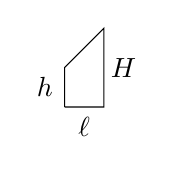
\begin{tikzpicture}[baseline=1.5ex]
        \draw (0, 0) -- (0.5, 0) -- (0.5, 1) -- (0, 0.5) -- (0, 0);
        \node at (0.25, -0.25) {$\ell$};
        \node at (0.75, 0.5) {$H$};
        \node at (-0.25, 0.25) {$h$};
    \end{tikzpicture}\hspace{1em} vaut $\dfrac{h+H}2\ell$. Pour le voir, 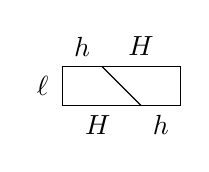
\begin{tikzpicture}[baseline=1ex]
        \draw (0, 0) -- (0, 0.5) -- (1.5, 0.5) -- (1.5, 0) -- (0, 0);
        \draw (1, 0) -- (0.5, 0.5);
        \node at (0.45, -0.25) {$H$};
        \node at (1.25, -0.25) {$h$};
        \node at (0.25, 0.75) {$h$};
        \node at (1, 0.75) {$H$};
        \node at (-0.25, 0.25) {$\ell$};
    \end{tikzpicture}
\end{rem}

On se donne $f\in\mathcal C^2([a, b], \mathbb R)$
\begin{center}
    \includegraphics{src/figures/integration-trapezes.pdf}
\end{center}
On note
    \[
        a_k=a+k\frac{b-a}n
    \]
et on va montrer que \[
    S_n(f)=\sum_{k=0}^{n-1}\frac{f(a_k)+f(a_{k+1})}2\times \frac{b-a}n
\]
approche l'intégrale et on va majorer l'erreur commise. Pour ça, on note \[
    g_k(x)=f(a_k)\frac{x-a_{k+1}}{a_k-a_{k+1}}+f(a_{k+1})\frac{x-a_k}{a_{k+1}-a_k}
\]
de sorte que \[
    \int_a^bf-S_n(f)=\sum_{k=0}^{n-1}\int_{a_k}^{a_{k+1}}f-g_k
\]
donc \[
    \left| \int_a^bf-S_n(f) \right|\leq \sum_{k=0}^{n-1}\int_{a_k}^{a_{k+1}}|f-g_k|.
\]
Pour $x\in]a_k, a_{k+1}[$, on note $\lambda\in\mathbb R$ tel que \[
    f(x)=g_k(x)+\frac\lambda2(x-a_k)(x-a_{k+1}).
\]
La fonction \[
    h:t\in[a_k, a_{k+1}]\longmapsto f(t)-g_k(t)-\frac\lambda2(t-a_k)(t-a_{k+1})
\]
s'annule en trois points donc en appliquant Rolle deux fois, il existe $\gamma$ tel que \[
    h''(\gamma)=0\implies \lambda=f''(\gamma)
\]
Par suite, \[
    |f(x)-g_k(x)|\leq \frac12\sup_{[a_k, a_{k+1}]}|f''|\cdot |(x-a_k)(x-a_{k+1})|
\]
d'où on tire \[
    \left| \int_a^bf-S_n(f) \right|\leq \frac12\|f''\|_{\infty}\sum_{k=0}^{n-1}\int_{a_k}{a_{k+1}}(a_k-t)(t-a_{k+1})\diff t=\|f''\|_{\infty}\frac{(b-a)^3}{12n^2}
\]

\begin{rem}
    La majoration est un $O \left( \frac1{n^2} \right)$, ce qui est meilleur que la méthode des rectangles.
\end{rem}

\endchapter
